\documentclass[12pt,a4paper,final]{article}

\usepackage{a4wide}
\usepackage{amssymb}
\usepackage[english]{babel}
\usepackage{color}
\usepackage[colorlinks=false,%
            pdfkeywords={OCaml, Just In Time compilation, machine code generation},%
            pdftitle={Just-In-Time Compilation of OCaml byte-code},%
            pdfauthor={Benedikt Meurer},%
            pdfsubject={},%
            pdfdisplaydoctitle=true]{hyperref}
\usepackage{tikz}
\usepackage{varwidth}

\usetikzlibrary{arrows}
\usetikzlibrary{trees}

\begin{document}

\title{%
  Just-In-Time Compilation of OCaml byte-code
}
\author{%
  Benedikt Meurer\\
  Compilerbau und Softwareanalyse\\
  Universit\"at Siegen\\
  D-57072 Siegen, Germany\\
  \url{meurer@informatik.uni-siegen.de}
}
\date{}
\maketitle
\begin{abstract}
  TODO
\end{abstract}


%% Introduction
\section{Introduction}

TODO


%% Performance
\section{Performance} \label{section:Performance}

\begin{table*}[h]
  \footnotesize
  \centering
  \begin{tabular}{l|rrrr|rrrrrr}
    \multicolumn{1}{l|}{\large invocation}
    & \multicolumn{4}{c|}{{\large time} (cpu sec.)}
    & \multicolumn{6}{c}{\large speedup}
    \\
    command
    & $t_{byt}$ & $t_{jit}$ & $t_{jit2}$ & $t_{opt}$
    & $\sigma^{jit}_{byt}$ & $\sigma^{jit2}_{byt}$ & $\sigma^{opt}_{byt}$
    & $\sigma^{jit2}_{jit}$ & $\sigma^{opt}_{jit}$ & $\sigma^{opt}_{jit2}$
    \\
    \hline
    \texttt{almabench} & $27.61$ & & $8.58$ & $4.47$ &  & $3.22$ & $6.17$ &  &  & $1.92$\\
    \texttt{almabench.unsafe} & $27.54$ &  & $6.14$ & $4.35$ &  & $4.48$ & $6.33$ &  &  & $1.41$\\
    \texttt{bdd} & $8.46$ &  & $2.00$ & $0.67$ &  & $4.23$ & $12.66$ &  &  & $2.99$\\
    \texttt{boyer} & $4.33$ &  & $1.66$ & $1.05$ &  & $2.61$ & $4.11$ &  &  & $1.57$\\
    \texttt{fft} & $5.69$ &  & $1.98$ & $0.64$ &  & $2.88$ & $8.96$ &  &  & $3.11$\\
    \texttt{nucleic} & $14.77$ &  & $3.24$ & $0.80$ &  & $4.56$ & $18.53$ &  &  & $4.06$\\
    \texttt{quicksort} & $6.78$ &  & $1.28$ & $0.23$ &  & $5.31$ & $29.22$ &  &  & $5.50$\\
    \texttt{quicksort.unsafe} & $4.07$ &  & $0.84$ & $0.19$ &  & $4.86$ & $21.07$ &  &  & $4.34$\\
    \texttt{soli} & $0.17$ &  & $0.04$ & $0.01$ &  & $4.81$ & $17.30$ &  &  & $3.60$\\
    \texttt{soli.unsafe} & $0.14$ &  & $0.02$ & $0.01$ &  & $6.85$ & $17.12$ &  &  & $2.50$\\
    \texttt{sorts} & $19.42$ &  & $7.24$ & $3.71$ &  & $2.68$ & $5.23$ &  &  & $1.95$\\
  \end{tabular}
  \caption{Running time and speedup (Intel Core 2 Duo, Mac OS X 10.6)}
  \label{table:Running_time_and_speedup_Intel_Core_2_Duo}
\end{table*}

\begin{table*}[h]
  \footnotesize
  \centering
  \begin{tabular}{l|rrrr|rrrrrr}
    \multicolumn{1}{l|}{\large invocation}
    & \multicolumn{4}{c|}{{\large time} (cpu sec.)}
    & \multicolumn{6}{c}{\large speedup}
    \\
    command
    & $t_{byt}$ & $t_{jit}$ & $t_{jit2}$ & $t_{opt}$
    & $\sigma^{jit}_{byt}$ & $\sigma^{jit2}_{byt}$ & $\sigma^{opt}_{byt}$
    & $\sigma^{jit2}_{jit}$ & $\sigma^{opt}_{jit}$ & $\sigma^{opt}_{jit2}$
    \\
    \hline
    \texttt{almabench} & $28.52$ &  & $9.40$ & $5.36$ &  & $3.03$ & $5.32$ &  &  & $1.76$\\
    \texttt{almabench.unsafe} & $26.52$ &  & $7.87$ & $5.56$ &  & $3.37$ & $4.77$ &  &  & $1.42$\\
    \texttt{bdd} & $9.51$ &  & $2.03$ & $0.59$ &  & $4.69$ & $16.23$ &  &  & $3.46$\\
    \texttt{boyer} & $3.77$ &  & $1.68$ & $1.02$ &  & $2.24$ & $3.70$ &  &  & $1.65$\\
    \texttt{fft} & $5.65$ &  & $1.47$ & $0.34$ &  & $3.85$ & $16.62$ &  &  & $4.32$\\
    \texttt{nucleic} & $14.00$ &  & $3.28$ & $0.78$ &  & $4.27$ & $17.86$ &  &  & $4.18$\\
    \texttt{quicksort} & $5.32$ &  & $1.26$ & $0.23$ &  & $4.23$ & $22.81$ &  &  & $5.39$\\
    \texttt{quicksort.unsafe} & $5.48$ &  & $0.88$ & $0.18$ &  & $6.25$ & $29.80$ &  &  & $4.77$\\
    \texttt{soli} & $0.14$ &  & $0.03$ & $0.01$ &  & $4.18$ & $15.33$ &  &  & $3.67$\\
    \texttt{soli.unsafe} & $0.12$ &  & $0.02$ & $0.01$ &  & $6.56$ & $16.86$ &  &  & $2.57$\\
    \texttt{sorts} & $21.50$ &  & $7.08$ & $3.61$ &  & $3.03$ & $5.96$ &  &  & $1.96$\\
  \end{tabular}
  \caption{Running time and speedup (Intel Xeon, CentOS 5.5)}
  \label{table:Running_time_and_speedup_Intel_Xeon}
\end{table*}

\begin{table*}[h]
  \footnotesize
  \centering
  \begin{tabular}{l|rrrr|rrrrrr}
    \multicolumn{1}{l|}{\large invocation}
    & \multicolumn{4}{c|}{{\large time} (cpu sec.)}
    & \multicolumn{6}{c}{\large speedup}
    \\
    command
    & $t_{byt}$ & $t_{jit}$ & $t_{jit2}$ & $t_{opt}$
    & $\sigma^{jit}_{byt}$ & $\sigma^{jit2}_{byt}$ & $\sigma^{opt}_{byt}$
    & $\sigma^{jit2}_{jit}$ & $\sigma^{opt}_{jit}$ & $\sigma^{opt}_{jit2}$
    \\
    \hline
    \texttt{almabench} & $57.72$ & $28.81$ & $20.09$ & $17.20$ & $2.00$ & $2.87$ & $3.35$ & $1.43$ & $1.67$ & $1.17$\\
    \texttt{almabench.unsafe} & $56.08$ & $26.04$ & $16.89$ & $19.70$ & $2.15$ & $3.32$ & $2.85$ & $1.54$ & $1.32$ & $0.86$\\
    \texttt{bdd} & $15.51$ & $6.25$ & $4.90$ & $1.14$ & $2.48$ & $3.17$ & $13.56$ & $1.28$ & $5.47$ & $4.28$\\
    \texttt{boyer} & $8.31$ & $4.30$ & $3.84$ & $1.96$ & $1.93$ & $2.16$ & $4.23$ & $1.12$ & $2.19$ & $1.96$\\
    \texttt{fft} & $13.70$ & $7.20$ & $5.23$ & $3.27$ & $1.90$ & $2.62$ & $4.19$ & $1.38$ & $2.20$ & $1.60$\\
    \texttt{nucleic} & $33.21$ & $14.65$ & $7.56$ & $2.11$ & $2.27$ & $4.39$ & $15.72$ & $1.94$ & $6.94$ & $3.58$\\
    \texttt{quicksort} & $10.93$ & $3.64$ & $3.10$ & $0.34$ & $3.00$ & $3.53$ & $32.14$ & $1.18$ & $10.72$ & $9.11$\\
    \texttt{quicksort.unsafe} & $9.15$ & $2.79$ & $2.16$ & $0.28$ & $3.28$ & $4.23$ & $32.67$ & $1.29$ & $9.96$ & $7.73$\\
    \texttt{soli} & $0.32$ & $0.08$ & $0.06$ & $0.02$ & $3.86$ & $5.40$ & $20.25$ & $1.40$ & $5.25$ & $3.75$\\
    \texttt{soli.unsafe} & $0.27$ & $0.06$ & $0.03$ & $0.01$ & $4.79$ & $9.57$ & $22.33$ & $2.00$ & $4.67$ & $2.33$\\
    \texttt{sorts} & $47.18$ & $20.62$ & $16.55$ & $6.26$ & $2.29$ & $2.85$ & $7.53$ & $1.25$ & $3.29$ & $2.64$\\
  \end{tabular}
  \caption{Running time and speedup (Intel Pentium 4, Debian testing)}
  \label{table:Running_time_and_speedup_Intel_Pentium_4}
\end{table*}

\begin{figure*}[h]
  \centering
  \footnotesize
  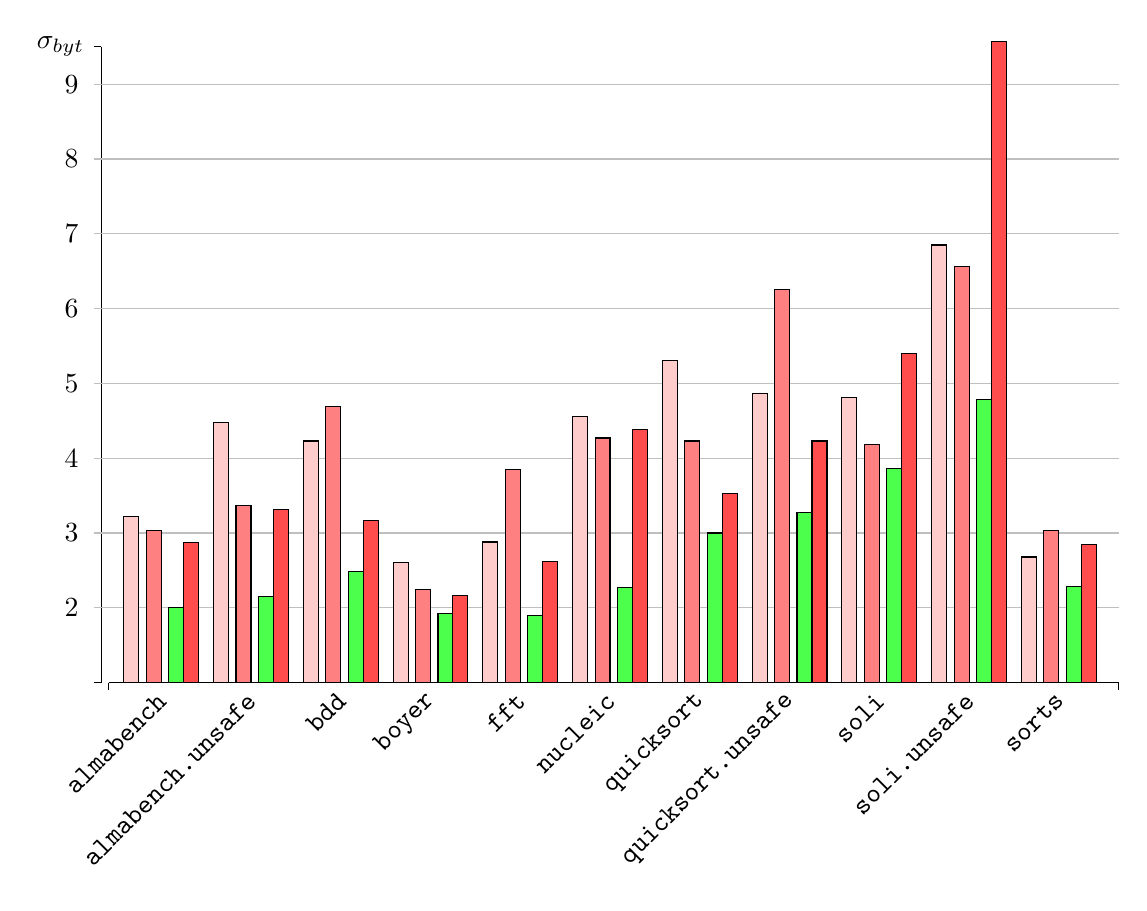
\begin{tikzpicture}[scale=.95]
    \definecolor{color}{HTML}{483D8B}
    \draw (0cm,0cm) -- (13.5cm,0cm);  %Abzisse
    \draw (0cm,0cm) -- (0cm,-0.1cm);  %linkes Ende der Abzisse
    \draw (13.5cm,0cm) -- (13.5cm,-0.1cm);  %rechtes Ende der Abzisse
    \draw (-0.1cm,0cm) -- (-0.1cm,8.5cm);  %Ordinate
    \draw (-0.1cm,0cm) -- (-0.2cm,0cm);  %unteres Ende der Ordinate
    \draw (-0.1cm,8.5cm) -- (-0.2cm,8.5cm) node [left] {$\sigma_{byt}$};  %oberes Ende der Ordinate
    \foreach \x in {2,...,9}
    {
      \draw[gray!50, text=black] (-0.2 cm,\x cm - 1cm) -- (13.5 cm,\x cm - 1cm) node at (-0.5 cm,\x cm - 1cm) {\x};
    }
    \foreach \name/\x/\a/\b/\c/\d in
    {
      almabench/0 / 3.22 / 3.03 / 2.00/2.87,
      almabench.unsafe/1 / 4.48 / 3.37 / 2.15/3.32,
      bdd/2 / 4.23 / 4.69 / 2.48/3.17,
      boyer/3 / 2.61 / 2.24 / 1.93/2.16,
      fft/4 / 2.88 / 3.85 / 1.90/2.62,
      nucleic/5 / 4.56 / 4.27 / 2.27/4.39,
      quicksort/6 / 5.31 / 4.23 / 3.00/3.53,
      quicksort.unsafe/7 / 4.86 / 6.25 / 3.28/4.23,
      soli/8 / 4.81 / 4.18 /  3.86/5.40,
      soli.unsafe/9 / 6.85 / 6.56 / 4.79/9.57,
      sorts/10 / 2.68 / 3.03 / 2.29/2.85
    }
    {
      \pgfmathsetmacro\xinc{0.2}
      \pgfmathsetmacro\xoff{\x * 1.2 + \xinc}
      \pgfmathsetmacro\aoff{\a - 1.0}
      \pgfmathsetmacro\boff{\b - 1.0}
      \pgfmathsetmacro\coff{\c - 1.0}
      \pgfmathsetmacro\doff{\d - 1.0}
      \draw[fill=red!20] (\xoff cm + 0 * \xinc cm, 0 cm) rectangle (1 * \xinc cm + \xoff cm, \aoff);
      \draw[fill=red!50] (\xoff cm + 1 * \xinc cm + .1cm, 0 cm) rectangle (2 * \xinc cm + \xoff cm + .1cm, \boff);
      \draw[fill=green!70] (\xoff cm + 2 * \xinc cm + .2cm, 0 cm) rectangle (3 * \xinc cm + \xoff cm + .2cm, \coff);
      \draw[fill=red!70] (\xoff cm + 3 * \xinc cm + .2cm, 0 cm) rectangle (4 * \xinc cm + \xoff cm + .2cm, \doff);
      \node[rotate=45,left] at (\xoff cm + 3 * \xinc cm, -.1cm) {\texttt{\name}};
    };
  \end{tikzpicture}
  \caption{Speedup relative to the byte-code interpreter}
  \label{figure:Speedup_relative_to_the_byte_code_interpreter}
\end{figure*}

\begin{figure*}[h]
  \centering
  \footnotesize
  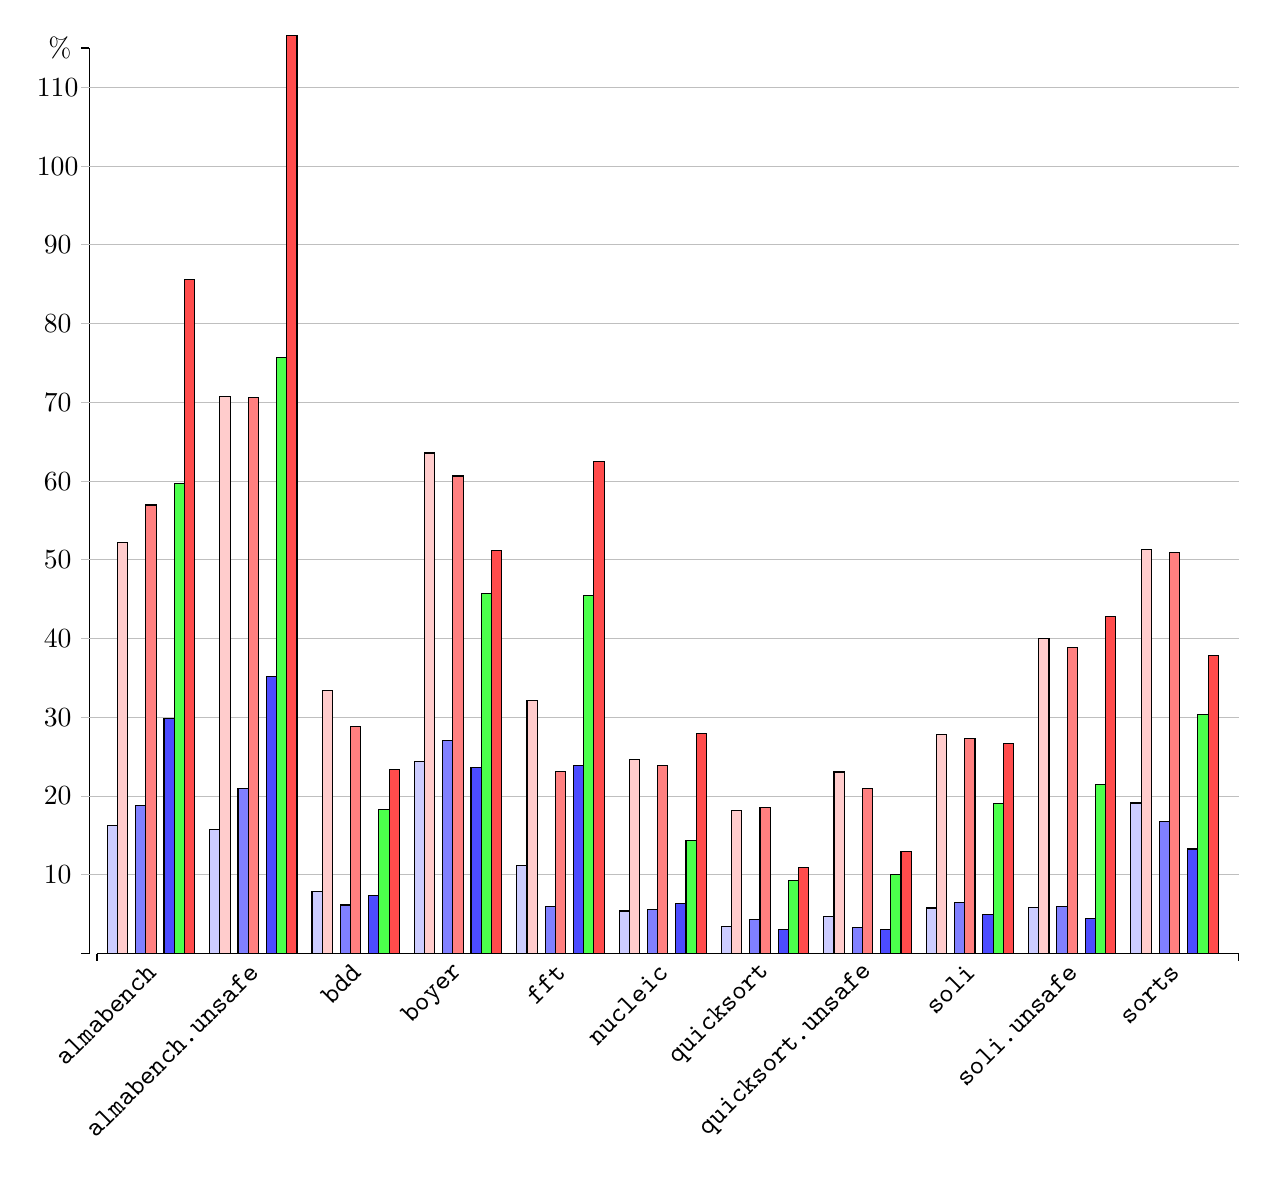
\begin{tikzpicture}
    \definecolor{color}{HTML}{483D8B}
    \draw (0cm,0cm) -- (14.5cm,0cm);  %Abzisse
    \draw (0cm,0cm) -- (0cm,-0.1cm);  %linkes Ende der Abzisse
    \draw (14.5cm,0cm) -- (14.5cm,-0.1cm);  %rechtes Ende der Abzisse
    \draw (-0.1cm,0cm) -- (-0.1cm,11.5cm);  %Ordinate
    \draw (-0.1cm,0cm) -- (-0.2cm,0cm);  %unteres Ende der Ordinate
    \draw (-0.1cm,11.5cm) -- (-0.2cm,11.5cm) node [left] {\%};  %oberes Ende der Ordinate
    \foreach \y in {1,...,11}  %Hilfslinien
    {
      \pgfmathtruncatemacro\ytext{\y * 10}
      \draw[gray!50, text=black] (-0.2 cm,\y cm) -- (14.5 cm,\y cm)
        node at (-0.5 cm,\y cm) {\ytext};  %Beschriftung
    };
    \foreach \name/\x/\a/\b/\c/\d/\e/\f/\g in
    {
      almabench/0 / 1.621/5.218 / 1.878/5.696 / 2.981/5.971/8.564,
      almabench.unsafe/1 / 1.579/7.079 / 2.097/7.065 / 3.513/7.567/11.662,
      bdd/2 / 0.790/3.340 / 0.616/2.888 / 0.738/1.830/2.337,
      boyer/3 / 2.435/6.357 / 2.703/6.065 / 2.363/4.572/5.115,
      fft/4 / 1.116/3.212 / 0.602/2.316 / 2.389/4.544/6.254,
      nucleic/5 / 0.540/2.461 / 0.560/2.390 / 0.636/1.441/2.794,
      quicksort/6 / 0.342/1.817 / 0.438/1.854 / 0.311/0.933/1.098,
      quicksort.unsafe/7 / 0.475/2.306 / 0.336/2.098 / 0.306/1.004/1.294,
      soli/8 / 0.578/2.778 / 0.652/2.727 / 0.494/1.905/2.667,
      soli.unsafe/9 / 0.584/4.000 / 0.593/3.889 / 0.448/2.143/4.286,
      sorts/10 / 1.912/5.131 / 1.679/5.095 / 1.328/3.038/3.785
    }
    {
      \pgfmathsetmacro\xinc{0.13}
      \pgfmathsetmacro\xoff{\x * 1.3 + \xinc}
      \draw[fill=blue!20] (\xoff cm + 0 * \xinc cm, 0 cm) rectangle (1 * \xinc cm + \xoff cm, \a);
      \draw[fill=red!20] (\xoff cm + 1 * \xinc cm, 0 cm) rectangle (2 * \xinc cm + \xoff cm, \b);
      \draw[fill=blue!50] (\xoff cm + 2 * \xinc cm + .1cm, 0 cm) rectangle (3 * \xinc cm + \xoff cm + .1cm, \c);
      \draw[fill=red!50] (\xoff cm + 3 * \xinc cm + .1cm, 0 cm) rectangle (4 * \xinc cm + \xoff cm + .1cm, \d);
      \draw[fill=blue!70] (\xoff cm + 4 * \xinc cm + .2cm, 0 cm) rectangle (5 * \xinc cm + \xoff cm + .2cm, \e);
      \draw[fill=green!70] (\xoff cm + 5 * \xinc cm + .2cm, 0 cm) rectangle (6 * \xinc cm + \xoff cm + .2cm, \f);
      \draw[fill=red!70] (\xoff cm + 6 * \xinc cm + .2cm, 0 cm) rectangle (7 * \xinc cm + \xoff cm + .2cm, \g);
      \node[rotate=45,left] at (\xoff cm + 5 * \xinc cm, -.1cm) {\texttt{\name}};
    };
  \end{tikzpicture}
  \caption{Performance relative to \texttt{ocamlopt}}
  \label{figure:Performance_relative_to_ocamlopt}
\end{figure*}



%% Future work
\section{Future work} \label{section:Future_work}

TODO


%% Conclusion
\section{Conclusion} \label{section:Conclusion}

TODO


%% Acknowlegdements
\section*{Acknowledgements}

TODO


%% References
\bibliographystyle{abbrv}
\bibliography{citations}

\end{document}
